%& -job-name=Curriculum Vitae
\documentclass[12pt]{article}
\usepackage[utf8]{inputenc}
\usepackage{fancyhdr}
\usepackage[document]{ragged2e}
\usepackage[a4paper,width=180mm,top=25mm,bottom=25mm]{geometry}
\usepackage{hyperref}
\hypersetup{
    colorlinks=true,
    linkcolor=blue,
    filecolor=magenta,
    urlcolor=cyan,
    }
\usepackage{float}
\usepackage{wrapfig}
\usepackage{graphicx}
\usepackage{blindtext}
\usepackage{multicol}
\usepackage{float}
\usepackage{paralist}
\usepackage{marvosym}
\usepackage{hologo}
\usepackage[compact]{titlesec}
\titlespacing{\section}{0pt}{2ex}{1ex}
\titlespacing{\subsection}{0pt}{2ex}{1ex}
\titlespacing{\subsubsection}{0pt}{2ex}{1ex}
\usepackage{emoji}
\setemojifont{TwemojiMozilla}
\renewcommand{\familydefault}{\sfdefault}
\begin{document}
\pagenumbering{gobble}




\textbf{\huge{Jelle Langedijk}}\\
\noindent\hfil\rule{\textwidth}{.4pt}\hfill\\
\vspace{0.5cm}
\begin{minipage}{0.6\textwidth}
\large
\emoji{mobile-phone}    \textit{Phone}      \hfill      $\cdots$\\
\emoji{email}           \textit{E-Mail}     \hfill      \textit{j.langedijk@student.tue.nl}\\
\emoji{desktop-computer} \textit{GitHub} \hfill \href{https://github.com/JelleLa}{GitHub Account}\\
\emoji{person-in-tuxedo-light-skin-tone}      \textit{LinkedIn}   \hfill      \href{https://www.linkedin.com/in/jelle-langedijk-a422281a0/}{LinkedIn Page}\\
\emoji{round-pushpin} \textit{Location} \hfill $\cdots$
\end{minipage}%
\hspace{1cm}
\begin{minipage}{0.4\textwidth}
\centering
%\includegraphics[width=0.5\linewidth]{example-image-a}
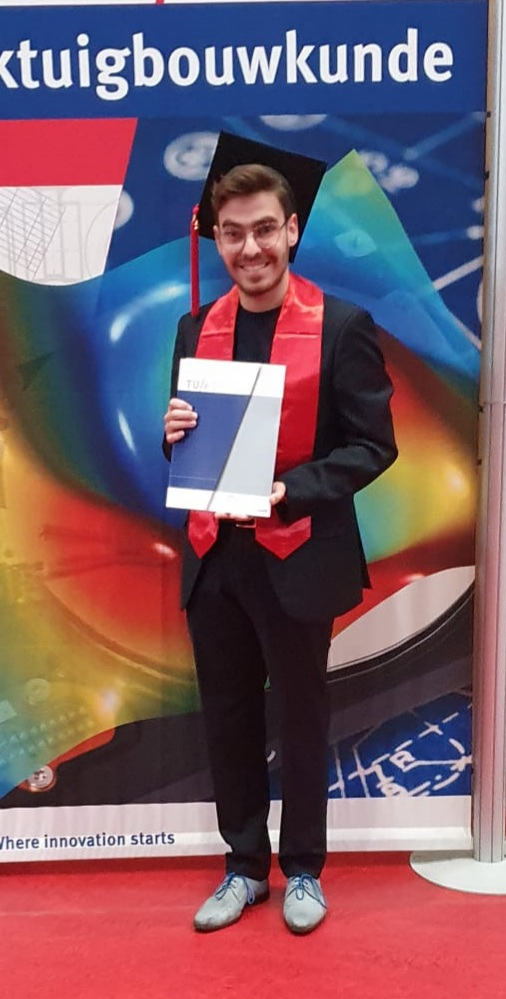
\includegraphics[trim=0 8cm 0 4cm,clip,width=0.5\linewidth]{IMG-20211016-WA0025.jpg}
\end{minipage}
\vspace{0.5cm}



\hfill\\

\textit{\huge{Education}} \\
\noindent\hfil\rule{\textwidth}{.4pt}\hfil

\textbf{Huygens Lyceum Eindhoven | \textit{Natuur en Techniek}} \hfill \textit{2012-2018}\\
Completed the final exam Atheneum in the program Nature \& Technology with favourable consequence. Graduated in the \textit{Dutch}, \textit{English} and \textit{French Language and Literature}, \textit{Mathematics (B \& D)}, \textit{Physics}, \textit{Chemistry} and \textit{Management and Organisation (MO)}.
\vspace{0.5cm}


\textbf{Eindhoven University Of Technology | \textit{BSc Mechanical Engineering}} \hfill \textit{2018-2021}\\
Completed the propaedeutic phase in the first academic year (2018-2019). Obtained Bachelors degree \textit{with great appreciation}, average grade of 7.6/10. Curriculum existed of courses in
\begin{compactitem}
    \item Dynamics of Mechanical Systems and Robotics;
    \item Control Systems;
    \item Material Science;
    \item Technology Entrepreneurship;
    \item Manufacturing Networks;
    \item Transport Phenomena (Fluid Dynamics, Heat, Flow).
\end{compactitem}
Bachelors End Project done in the \textit{Dynamics and Control} group, see \textit{Projects}.

\vspace{0.5cm}

\textbf{Eindhoven University Of Technology | \textit{MSc Mechanical Engineering at the Dynamics and Control Group (Special track Manufacturing Systems Engineering)}} \hfill \textit{2021-present}\\
Curriculum consists of courses in
\begin{compactitem}
    \item Acoustics: \textit{vibration isolation, structure-borne sound, sound radiation, propagation and sound imaging};
    \item Classic Dynamics: \textit{linear, nonlinear, multi-body, switching};
    \item Network Dynamics: \textit{consensus, cooperation, sensor allocation};
    \item Control: \textit{linear, nonlinear, Design Structure Matrix Modeling};
    \item Manufacturing Networks: \textit{discrete models, stochastic models, dynamical models, queuing theory};
    \item Mathematics: \textit{(systems of) Ordinary Differential Equations, Partial Differential Equations};
    \item Data Analytics: \textit{Machine Learning (Supervised,Unsupervised), Neural Networks};
    \item Manufacturing Technology;
    \item Fracture Mechanics.

\end{compactitem}
Expected to complete all courses within the first academic year (2021-2022). Average as of 31/05/2022: 8.3/10.


\hfill\\

\textit{\huge{Skills}} \\
\noindent\hfil\rule{\textwidth}{.4pt}\hfill

\textbf{Engineering}\\
\begin{multicols}{2}
\begin{compactitem}
    \item \textit{Classic Dynamics}
    \item \textit{Network \& Cooperation Dynamics}
    \item \textit{Switching Dynamics}
    \item \textit{Structural Dynamics}
    \item \textit{Signal Processing}
    \item \textit{Acoustics}
    \item \textit{Linear \& Nonlinear Control}
    \item \textit{Manufacturing Network Modeling}
    \item \textit{Modeling of Manufacturing Processes}
    \item \textit{Machine Learning}
    \item \textit{Fracture Mechanics}
\end{compactitem}
\end{multicols}

\textbf{Software and Programming, Scripting and Typesetting Languages}\\

\begin{multicols}{3}
\begin{compactitem}
    \item \textit{MATLAB, GNU Octave}
    \item \textit{Simulink}
    \item \textit{Python}
    \item \textit{Siemens NX 12}
    \item \textit{\LaTeXe, \hologo{pdfLaTeX}, \hologo{LuaLaTeX}}
    \item \textit{Markdown, R Markdown}
    \item \textit{PGF/TikZ}
    \item \textit{GNU+Linux}
    \item \textit{Bash}
    \item \textit{Mentat \& Marc}
\end{compactitem}
\end{multicols}


\textbf{Soft Skills}\\

\begin{multicols}{2}
\begin{compactitem}
    \item (Inter-Disciplinary) Teamwork
    \item Time Management
    \item Critical Thinking
    \item Working independently and proactively with high self-discipline
\end{compactitem}
\end{multicols}

\textit{\huge{Projects}} \\
\noindent\hfil\rule{\textwidth}{.4pt}\hfil

\begin{compactitem}
    % \item Truss Structure Design and Optimisation using \textit{Mentat and Marc};
    % \item Trebuchet Design and Simulation using \textit{Siemens NX 12 and Simcenter 12};
    % \item Peristaltic Pump Design using servo motors controlled with an \textit{Arduino} and \textit{MATLAB};
    % \item Solar Heat System Design on a low budget. Heat Transfer Model made in \textit{MATLAB};
    \item Simulating Skyscrapers during an earthquake with a pendulum. Physical model verified with a numerical model in \textit{MATLAB};
    % \item Modelled the LaGrange Dynamics and Control for a Luffing Crane in \textit{MATLAB};
    % \item Numerically modelled an Ideal and Real thermodynamic cycle of a combustion engine in \textit{MATLAB};
    % \item Modelled the (Inverse) Kinematics, Dynamics and Control Design of a robot arm in \textit{MATLAB};
    % \item Worked out a business model and plan for an alternative solution to proctoring software;
    % \item Identification and shifting of problematic eigenmodes of a Canon Colorado 1650 printer using \textit{Siemens NX 12 Nastran};
    % \item Modeling and controlling of a Distribution and Handling Station in \textit{CIF}
    % \item Designing a mobile camera crane for the film industry. Design verified using \textit{MATLAB}. Design drawn (3D and technical drawings) in \textit{Siemens NX 12};
    \item Consulted \textit{Vanderlande} in business model innovation for their new  \href{https://www.vanderlande.com/evolutions/fleet/}{AGV Fleet} technology for airport logistics;
    \item Bachelor End Project: Developing a Discrete-Event Simulation toolbox in \textit{Python} as alternative to the TU/e's current software package $\chi3$. Supervisor: \href{https://www.tue.nl/en/research/researchers/erjen-lefeber/}{A.A.J. Lefeber}. Graded 9/10; 10/10 for my self-reliance and professional behavior. Paper publicly available \href{https://dc.wtb.tue.nl/lefeber/do_download_pdf.php?id=288}{here}.
\end{compactitem}
\vspace{0.5cm}

\textit{\huge{Work Experience}} \\
\noindent\hfil\rule{\textwidth}{.4pt}\hfil

\textbf{Shop Assistant at Kruidvat}\hfill \textit{2014-2017}\\
Worked as both a shop assistant as well as a stock clerk.\\
\hfill\\
\textbf{Employee at Washin7 Eindhoven}\hfill \textit{2018-Present}\\
Work as a car wash employee with many functions, like cashier, guiding cars in the automatic car wash, operating the car wash, damage reporting, cleaning and recently leading a team with full responsibility.\\
\hfill\\
\textbf{Volunteer at Huygens Lyceum Eindhoven}\hfill \textit{2019,2022}\\
Volunteered at the \textit{"tafeltjesavond"} event twice as alumni, where I helped high-school students by making their choice of follow-up education.
\vspace{0.5cm}

\newpage
\textit{\huge{Hobbies}} \\
\noindent\hfil\rule{\textwidth}{.4pt}\hfill
\begin{compactitem}
    \item I collect HIFI audio gear, as well as music in different formats like Records, Cassettes and High Bitrate FLAC's. I'm always in search to optimise any aspect of my system with the knowledge I have;
    %\item I play bi-weekly Dungeons and Dragons with a group of friends;
    \item Since I'm an advocate for Free Open Source Software, I often tinker around with GNU+Linux to optimise my workflow and learn new things.
\end{compactitem}

\end{document}

